%%%%%%%%%%%%%%%%%%%%%%%%%%%%%%%%%%%%%%%%%%%%%%%%%%%%%%%%%%%%%%%%%%%%%%%%%%%%%%%%%%%%%%%%%%%%%%%%%%%%%%%%%%%
%                                           PACKAGES                                                      %
%%%%%%%%%%%%%%%%%%%%%%%%%%%%%%%%%%%%%%%%%%%%%%%%%%%%%%%%%%%%%%%%%%%%%%%%%%%%%%%%%%%%%%%%%%%%%%%%%%%%%%%%%%%
\documentclass[12pt, fleqn]{article}
\usepackage{amsmath, amsfonts, amsthm, amssymb, graphicx, enumitem, mathtools, MnSymbol, relsize, cancel}
\usepackage{siunitx}
\DeclareSIUnit\angstrom{\text{\AA}}
\usepackage{pdfpages}
\usepackage{graphicx}
\usepackage[utf8]{inputenc}
\usepackage{biblatex}
\usepackage{pythontex}
\usepackage{listings}
\usepackage[pdftex,pdfpagelabels,bookmarks,hyperindex,hyperfigures]{hyperref}
\hypersetup{colorlinks=true,allcolors=blue}
\usepackage{hypcap}
\usepackage{float}
\usepackage{geometry}
\geometry{margin=1in}
%%%%%%%%%%%%%%%%%%%%%%%%%%%%%%%%%%%%%%%%%%%%%%%%%%%%%%%%%%%%%%%%%%%%%%%%%%%%%%%%%%%%%%%%%%%%%%%%%%%%%%%%%%%
%                                           REFERENCE FILE                                                %
%%%%%%%%%%%%%%%%%%%%%%%%%%%%%%%%%%%%%%%%%%%%%%%%%%%%%%%%%%%%%%%%%%%%%%%%%%%%%%%%%%%%%%%%%%%%%%%%%%%%%%%%%%%
\usepackage[export]{adjustbox}
\graphicspath{{images/}}
%%%%%%%%%%%%%%%%%%%%%%%%%%%%%%%%%%%%%%%%%%%%%%%%%%%%%%%%%%%%%%%%%%%%%%%%%%%%%%%%%%%%%%%%%%%%%%%%%%%%%%%%%%%
%                                          PREPARE TITLE AND ABSTRACT                                     %
%%%%%%%%%%%%%%%%%%%%%%%%%%%%%%%%%%%%%%%%%%%%%%%%%%%%%%%%%%%%%%%%%%%%%%%%%%%%%%%%%%%%%%%%%%%%%%%%%%%%%%%%%%%
\title {
    \normalsize{UC Berkeley}\\
    \large{{EE140: Analog Integrated Circuit Devices\\Fall 2022\\Professor Ricky Muller\\}}
    \vspace{0.5ex}
    \Huge{Homework 2}
    \vspace{0.5ex}
}
\addbibresource{references.bib}
\author{Tarik Fawal}
\date{9 September 2022}
\usepackage{array}
\newcolumntype{C}[1]{>{\centering\arraybackslash}m{#1}}
\newcolumntype{N}{@{}m{0pt}@{}}
\begin{document}
%%%%%%%%%%%%%%%%%%%%%%%%%%%%%%%%%%%%%%%%%%%%%%%%%%%%%%%%%%%%%%%%%%%%%%%%%%%%%%%%%%%%%%%%%%%%%%%%%%%%%%%%%%%
%                                           GENERATE TITLE                                                %
%%%%%%%%%%%%%%%%%%%%%%%%%%%%%%%%%%%%%%%%%%%%%%%%%%%%%%%%%%%%%%%%%%%%%%%%%%%%%%%%%%%%%%%%%%%%%%%%%%%%%%%%%%%
\maketitle
\tableofcontents
\flushbottom
    \section*{Preface}
        \textit{\emph{This homework submission was created using \LaTeX.  The answers to questions were obtained through the course website, notes, textbook, and lecture videos.  I pledge that I have not plagiarized my solutions in any way, and the work presented here is my own.  References to any sources of material used in the solutions to this problem set are included at the end of this document.}}
%%%%%%%%%%%%%%%%%%%%%%%%%%%%%%%%%%%%%%%%%%%%%%%%%%%%%%%%%%%%%%%%%%%%%%%%%%%%%%%%%%%%%%%%%%%%%%%%%%%%%%%%%%%
%                                           QUESTION 1                                                    %
%%%%%%%%%%%%%%%%%%%%%%%%%%%%%%%%%%%%%%%%%%%%%%%%%%%%%%%%%%%%%%%%%%%%%%%%%%%%%%%%%%%%%%%%%%%%%%%%%%%%%%%%%%%
\newpage
\section{MOS Operating Points}
\textbf{\emph{Given: }} Different circuit topologies, with all transistors ($NMOS$ and $PMOS$) having the following set of properties:

    \begin{table}[H]
    \centering
    \setlength{\tabcolsep}{20pt}
    \renewcommand{\arraystretch}{1.5}
        \begin{tabular}{|l|c|}
            \hline
            $W$ & $10\,\mu m$\\
            \hline
            $L$ & $0.5\,\mu m$\\
            \hline
            $\mu C_{ox}$ & $200\,\mu A/V^2$\\
            \hline
            $\lambda$ & $0\,V^{-1}$\\
            \hline
            $\left|V_{th}\right|$ & $0.5\,V$\\
            \hline
        \end{tabular}
    \end{table}

\noindent
\textbf{\emph{Find: }} The following for each circuit:

\begin{enumerate}[label=(\roman*)]
    \item{The region of operation.}
    \item{The drain current, $I_D$.}
    \item{The drain-source voltage, $V_{DS}$.}
\end{enumerate}

\newpage\noindent
\textbf{\emph{Solution: }}The regions of operation are determined with reference to \textit{Table~\ref{tab:mosfet_op}}.

\begin{enumerate}[label=(\alph*)]
    %%%%%%%%%%%%%%%%%%
    %%% SOLUTION A %%%
    %%%%%%%%%%%%%%%%%%
    \item
    {
    Below is the given circuit:\\
    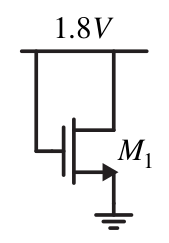
\includegraphics[scale=0.55, center]{p1a.png}\\
    \begin{enumerate}[label=(\roman*)]
        \item
        {
        \underline{\textbf{Region of Operation}}
        
        \vspace{0.15cm}
        This is an $NMOS$ transistor, with $V_{GS} = V_{DS} = 1.8\,V$.  Because $V_{GS} > V_{T_n} = 0.5\,V$, the transistor is on.  Furthermore, $V_{DS} = 1.8\,V > V_{GS} - V_{T_n} = 1.3\,V$, and this will always be the case since the drain and gate are both tied to the voltage source rail.
        
        \vspace{0.25cm}
        $\boxed{\therefore\quad{\text{The device is in \textit{saturation}.}}}$
        }
        \vspace{0.25cm}
        \item
        {
        \underline{\textbf{Drain Current, $I_D$}}
        
        \vspace{0.15cm}
        Because this is a saturated $NMOS$, we will use \textit{Eq.~\ref{eq:mosfet_ids_nmos_sat}} to solve for the drain current:
        \begin{align*}
            I_{DS,sat} &= \left(\frac{W}{2L}\right) \mu_n\,C_{ox}
                             {\big(V_{GS} - V_{T_n}\big)}^2 (1 + \cancelto{0}{\lambda V_{DS}})\\[0.25cm]
            &= \left(\frac{10\,\cancel{\mu m}}{2 \cdot 0.5\,\cancel{\mu m}}\right) 200\,\mu A/V^2{\big(1.3\,V\big)}^2\\[0.25cm]
            &= 10 \cdot 200\,\mu A/\cancel{V^2} \cdot 1.69\,\cancel{V^2}\\[0.25cm]
            &= 3380\,\mu A\\[0.25cm]
            \Aboxed{&= 3.38\,mA}
        \end{align*}
        }
        \item
        {
        \underline{\textbf{Drain-source Voltage, $V_{DS}$}}
        
        \vspace{0.15cm}
        As already noted, the drain-source voltage is $\boxed{V_{DS} = 1.8\,V}$.
        }
    \end{enumerate}
    }
    \newpage\noindent
    %%%%%%%%%%%%%%%%%%
    %%% SOLUTION B %%%
    %%%%%%%%%%%%%%%%%%
    \item
    {
    Below is the given circuit:\\
    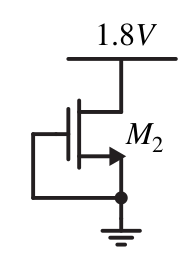
\includegraphics[scale=0.55, center]{p1b.png}\\
    \begin{enumerate}[label=(\roman*)]
        \item
        {
        \underline{\textbf{Region of Operation}}
        
        \vspace{0.15cm}
        This is also an $NMOS$ transistor, but now the gate is tied to ground. Because $V_{GS} \not > V_{T_n} = 0.5\,V$, the transistor is off.  Furthermore, since it is tied to ground this will always be the case.
        
        \vspace{0.25cm}
        $\boxed{\therefore\quad{\text{The device is in \textit{cut-off}.}}}$
        }
        \vspace{0.25cm}
        \item
        {
        \underline{\textbf{Drain Current, $I_D$}}
        
        \vspace{0.15cm}
        Because the device is off $\boxed{I_{DS} = 0\,A}$:
        }
        \vspace{0.25cm}
        \item
        {
        \underline{\textbf{Drain-source Voltage, $V_{DS}$}}
        
        \vspace{0.15cm}
        The drain-source voltage is $\boxed{V_{DS} = 1.8\,V}$.
        }
    \end{enumerate}
    }
    \newpage\noindent
    %%%%%%%%%%%%%%%%%%
    %%% SOLUTION C %%%
    %%%%%%%%%%%%%%%%%%
    \item
    {
    Below is the given circuit:\\
    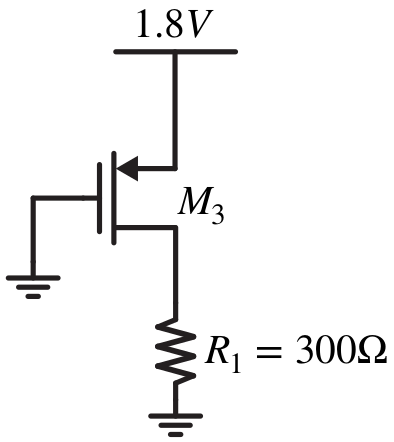
\includegraphics[scale=0.35, center]{p1c.png}\\
    \begin{enumerate}[label=(\roman*)]
        \item
        {
        \underline{\textbf{Region of Operation}}
        
        \vspace{0.15cm}
        This is a $PMOS$ transistor, with $V_{SG} = 1.8\,V$.  This exceeds the threshold voltage, so we know the device is on.  However, we don't know $V_D$, so we will assume saturation to solve for it, and then check our assumption.
        
        \vspace{0.15cm}
        Equating the current through $R_1$ to the drain current, we have:
        \begin{align*}
            I_{SD,sat} = \frac{V_D}{R_1}
            &=\left(\frac{W}{2L}\right) \mu_p\,C_{ox}{\big(V_{SG} - \left|V_{T_p}\right|\big)}^2\\[0.25cm]
            \Longrightarrow V_D &= R_1 \left[\left(\frac{W}{2L}\right) \mu_p\,C_{ox}{\big(V_{SG} - \left|V_{T_p}\right|\big)}^2\right]\\[0.25cm]
            &= (300\,\Omega) \left[\left(10\right) (200\,\mu A/V^2{(1.8\,V - 0.5\,V)}^2\right]\\[0.25cm]
            &= (300\,\Omega) \left[(2000\,\mu A) (1.69)\right]\\[0.25cm]
            \Aboxed{V_D &= 1.014\,V}
        \end{align*}
        
        Our result for $V_D$ tells us that $V_{SD} = 1.8\,V - 1.014\,V = 0.786\,V < V_{SG} - \left|V_{T_p}\right| = 1.3\,V$.  This contradicts the condition for the device being in saturation, which tells us that it is not operating in this region.
        
        \vspace{0.25cm}
        $\boxed{\therefore\quad{\text{The device is in \textit{triode}.}}}$
        }
        \newpage
        \item
        {
        \underline{\textbf{Drain Current, $I_D$}}
        
        \vspace{0.15cm}
        To solve for the drain current we first solve for the drain voltage using the same method in part (\textit{i}), but this time using the triode current:
        
        \begin{align*}
            I_{SD,tri} = \frac{V_D}{R_1}
            &=\left(\frac{W}{L}\right) \mu_p\,C_{ox}
                            \left(V_{SG} - \left|V_{T_p}\right| - \frac{V_{SD}}{2}\right) V_{SD}\\[0.25cm]
            \Longrightarrow V_D &= \left[\underbrace{\left(\frac{R_1\,W\,\mu_p\,C_{ox}}{L}\right)}_\phi \left(V_{SG} - \left|V_{T_p}\right| - \frac{V_{SD}}{2}\right)\right]  V_{SD}\\[0.25cm]
            &= \phi \left(1.3\,V - \frac{1.8\,V}{2} + \frac{V_D}{2}\right)\left(V_S - V_D\right)\\[0.25cm]
            \Longrightarrow \cancelto{1}{\frac{V_D}{V_D}} &= \phi \left(\frac{1.8\,V}{V_D} - \frac{1.8\,V}{2\,V_D} + \frac{1}{2}\right)\left(\frac{1.3\,V}{V_D} - 1\right)\\[0.25cm]
            &= \phi \left(\frac{2.6\,V + 1.8\,V + V_D}{2\,V_D}\right) \left(\frac{1.8\,V - V_D}{V_D}\right)\\[0.25cm]
            \Longrightarrow 2\,{V_D}^2 &= \phi \left(4.4\,V + V_D\right) \left(1.8\,V - V_D\right)\\[0.25cm]
            &= -\phi {V_D}^2 - 2.6\phi V_D + \phi7.92\\[0.25cm]
            \Longrightarrow 0 &= \underbrace{(2 + \phi)}_A\,{V_D}^2 + \underbrace{(2.6\phi)}_B\,V_D - \underbrace{7.92\phi}_C
        \end{align*}

        We now have a quadratic equation to use in order to solve for $V_D$.  Plugging the device parameters of $\phi$ yields the quadratic equation:
        \begin{equation}
            \boxed{3.2\,{V_D}^2 + 3.12\,V_D - 9.504 = 0}
        \end{equation}
        
        \vspace{0.25cm}
        Solving the equation with WolframAlpha yields two solutions, which is that either $V_D = -2.28\,V$, or $V_D = 1.3\,V$.  The negative voltage would give a negative drain voltage and undesirable transconductance.  The second positive voltage adheres to the conditions for the device to be operating in the triode region.  Thus, we choose $V_D = 1.3\,V$, which means that $V_{SD} = 0.7\,V$.
        
        \vspace{1cm}
        \noindent
        On the following page, we can now solve for the drain current.
        
        \newpage
        With reference to \textit{Eq.~\ref{eq:mosfet_ids_pmos_tri}}:
        \begin{align*}
            I_{SD,tri} &=\left(\frac{W}{L}\right) \mu_p\,C_{ox}
                            \left(V_{SG} - \left|V_{T_p}\right| - \frac{V_{SD}}{2}\right) V_{SD}\\[0.25cm]
            &=\left(20\right) 200 \mu A/V^2 \left(1.3\,V - \frac{0.7\,V}{2}\right) 0.7\,V\\[0.25cm]
            &= 4000 \mu A/V^2 \left(0.95\,V\right) 0.7\,V\\[0.25cm]
            &= 0.00266\,A
        \end{align*}
        \vspace{0.15cm}
        $\boxed{\therefore\quad{\text{This device has a drain current of : }I_{SD} = 2.66\,mA}}$
        }
        \vspace{0.25cm}
        \item
        {
        \underline{\textbf{Drain-source Voltage, $V_{SD}$}}
        
        \vspace{0.15cm}
        As already noted, the drain-source voltage is : $\boxed{V_{SD} = 0.7\,V}$
        }
    \end{enumerate}
    }
    \newpage\noindent
    %%%%%%%%%%%%%%%%%%
    %%% SOLUTION D %%%
    %%%%%%%%%%%%%%%%%%
    \item
    {
    Below is the given circuit:\\
    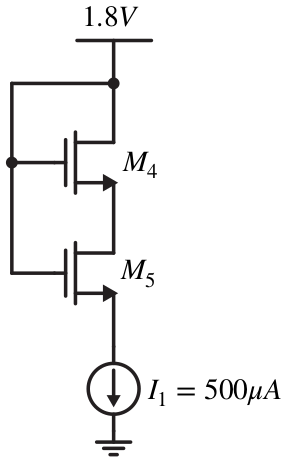
\includegraphics[scale=0.55, center]{p1d.png}\\
    \begin{enumerate}[label=(\roman*)]
        \item
        {
        \underline{\textbf{Region of Operation}}
        
        \vspace{0.15cm}
        This is a series $NMOS$ setup, with the transistor $M_4$ being diode-connected. One property of a diode-connected transistor is that it is always in saturation.  The gate of $M_5$ is also tied to the supply rail, so we know that it will exceed the threshold voltage and be turned on.  However, this one will be operating in the triode region.  The reason for this is because ${V_{D_5}}$ cannot larger than or equal to $0.5\,V$, or the top transistor would go into cut-off mode, which contradicts the condition that it must be in saturation.  Since there is no voltage drop across an ideal current source, with ${V_{DS_5}} < 0.5\,V$, $M_5$ cannot be in saturation.
        
        \vspace{0.25cm}
        $\boxed{\therefore\quad{\text{$M_4$ is in \textit{saturation}, $M_5$ is in \textit{triode}.}}}$
        }
        \vspace{0.25cm}
        \item
        {
        \underline{\textbf{Drain Current, $I_D$}}
        
        \vspace{0.15cm}
        We know that the constant current source, $I_1$ will bias the drain current of both $NMOS$ to be equal to the specified current of $500\,\mu A$.
        
        \vspace{0.25cm}
        $\boxed{\therefore\quad {I_{DS}}_4,sat = {I_{DS}}_5,tri = 500\,\mu A}$
        \vspace{0.25cm}
        }
        \newpage\noindent
        \item
        {
        \underline{\textbf{Drain-source Voltage, $V_{DS}$}}
        
        \vspace{0.15cm}
        We can use the fact that we know the drain current and the region of operation for each transistor to solve for ${V_{DS}}_4$ and ${V_{DS}}_5$.
        
        \vspace{0.25cm}
        Starting with the saturation current of $M_4$ (\textit{Eq.~\ref{eq:mosfet_ids_nmos_sat}}, and plugging in the given values:
        \begin{equation*}
            {I_{DS}}_4,sat = 10 \cdot 200\,\mu A/V^2 \cdot {\big({V_{GS}}_4 - 0.5\,V\big)}^2 = 500\,\mu A
        \end{equation*}
        Rearranging, and solving for ${V_{GS}}_4$:
        \begin{equation*}
            {V_{GS}}_4 = \sqrt{\frac{500\,\mu A}{2000\,\mu A/V^2}} + 0.5\,V = 1\,V
        \end{equation*}
        Now we can solve for ${V_S}_4$, which is also ${V_D}_5$:
        \begin{align*}
            {V_{GS}}_4 &= {V_G}_4 - {V_S}_4 = 1\,V\\[0.25cm]
            &\Longrightarrow {V_S}_4 = {V_G}_4 - 1\,V = 1.8\,V - 1\,V\\[0.25cm]
            \Aboxed{&= 0.8\,V}
        \end{align*}
        $\boxed{\therefore\quad V_{{DS}_4} = 1\,V}$
        }
        
        \vspace{0.5cm}
        The only unknown left is ${V_S}_5$.  We will use the triode current of $M_5$ to solve for it:
        \begin{align*}
            500\,\mu A &= 20 \cdot 200\,\mu A/V^2 \cdot \big({V_{GS}}_5 - V_T - \frac{{V_{DS}}_5}{2}\big){V_{DS}}_5 \\[0.25cm]
            &= 4000\,\mu A/V^2 \cdot \big({V_G}_5 - {V_S}_5 - V_T - \frac{{V_D}_5}{2} + \frac{{V_S}_5}{2}\big)({V_D}_5 - {V_S}_5) \\[0.25cm]
            &= 4000\,\mu A/V^2 \cdot \big(1.8 - {V_S}_5 - 0.5 - \frac{0.8}{2} + \frac{{V_S}_5}{2}\big)(0.8 - {V_S}_5)\\[0.25cm]
            &= 4000\,\mu A/V^2 \cdot (0.9 - \frac{{V_S}_5}{2})(0.8 - {V_S}_5)\\[0.25cm]
            &\Longrightarrow \frac{500\,\mu A}{4000\,\mu A/V^2} = (0.9)(0.8) - 0.9\,{V_S}_5 - \frac{0.8}{2}\,{V_S}_5 + \frac{{{V_S}_5}^2}{2}\\[0.25cm]
            &\Longrightarrow \frac{{{V_S}_5}^2}{2} -1.7\,{V_S}_5 + 0.845 = 0
        \end{align*}
        
        Solving the above quadratic equation yields two solutions for ${V_S}_5$, which are either $2.8\,V$ or $0.6\,V$.  Since the larger value yields a negative drain voltage, we choose the smaller value which also satisfies the condition for being in triode.
        
        \vspace{0.5cm}
        $\boxed{\therefore\quad V_{{DS}_5} = 0.2\,V}$
    \end{enumerate}
    }
    \newpage\noindent
    %%%%%%%%%%%%%%%%%%
    %%% SOLUTION E %%%
    %%%%%%%%%%%%%%%%%%
    \item
    {
    Below is the given circuit:\\
    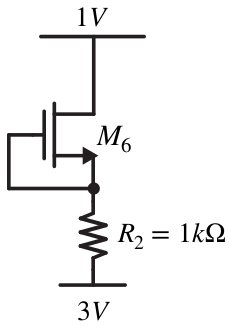
\includegraphics[scale=0.55, center]{p1e.png}\\
    \begin{enumerate}[label=(\roman*)]
        \item
        {
        \underline{\textbf{Region of Operation}}
        
        \vspace{0.15cm}
        This is a diode connected $NMOS$.
        
        $\boxed{\therefore\quad{\text{$M_6$ is in \textit{saturation}.}}}$
        }
        \vspace{0.25cm}
        \item
        {
        \underline{\textbf{Drain Current, $I_D$}}
        
        \vspace{0.15cm}
        The current across the resistor is equal to the saturation drain current:
        \begin{equation}
            I_D = \frac{3V - V_G}{R_2} = \left(\frac{W}{2L}\right) \mu_n\,C_{ox} {\big(V_{GS} - V_{T_n}\big)}^2
        \end{equation}
        Rearranging in terms of $V_G$:
        \begin{align*}
            -V_G &= \left[\underbrace{\left(\frac{R_2\,W}{2L}\right) \mu_n\,C_{ox}}_\phi {\big(V_{GS} - V_{T_n}\big)}^2\right] - 3\,V\\[0.25cm]
            &\Longrightarrow 0 = V_G + \phi({V_G}^2 - 1 - 2\,V_G + 2 + {V_T}^2) - 3\,V\\[0.25cm]
            &\Longrightarrow \underbrace{\phi}_A {V_G}^2 - \underbrace{2\phi}_B\,V_G + \underbrace{({V_T}^2 + \phi - 3)}_C = 0
        \end{align*}
        }
        Plugging in values for $\phi$ and $V_T$ yields the quadratic equation:
        
        \begin{equation}
            2\,{V_G}^2 - 4\phi\,V_G - 0.75 = 0
        \end{equation}
        
        There are two solutions, one of which is negative.  Since a negative gate voltage would violate the conditions for saturation (the transistor would be in cut-off), we choose the positive solution of $V_G = 2.17\,V$.
        
        \vspace{0.25cm}
        Now we can plug in values to solve for the drain current:
        \begin{align*}
            I_D &= \left(\frac{W}{2L}\right) \mu_n\,C_{ox} {\big(V_{GS} - V_{T_n}\big)}^2\\[0.25cm]
            &= \left(10 \cdot 200\,\mu A/V^2\right) {\big(1.17\,V - 0.5\,V\big)}^2\\[0.25cm]
            \Aboxed{&= 0.8978\,mA}
        \end{align*}
        \item
        {
        \underline{\textbf{Drain-source Voltage, $V_{DS}$}}
        
        \vspace{0.15cm}
        Since $V_G = V_D$, the drain voltage is : $\boxed{V_{DS} = 1.17\,V}$
        }
    \end{enumerate}
    }
    \newpage\noindent
    %%%%%%%%%%%%%%%%%%
    %%% SOLUTION F %%%
    %%%%%%%%%%%%%%%%%%
    \item
    {
    Below is the given circuit:\\
    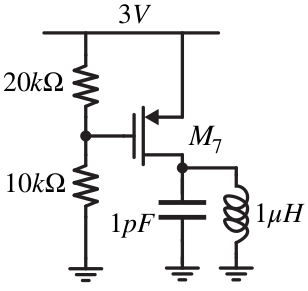
\includegraphics[scale=0.55, center]{p1f.png}\\
    \begin{enumerate}[label=(\roman*)]
        \item
        {
        \underline{\textbf{Region of Operation}}
        
        \vspace{0.15cm}
        This is a $DC$ circuit with a $PMOS$ transistor.  There is no current going into the gate of the MOSFET, so we can easily calculate the current traveling through both resistors:
        \begin{equation*}
            I_R = \frac{3\,V}{10\,k\Omega + 20\,k\Omega} = \frac{3\,V}{30\,k\Omega} = 0.1\,mA
        \end{equation*}
        Then the gate voltage is simply the drop across the $20\,k\Omega$ resistor subtracted from the supply rail:
        \begin{equation*}
            V_G = 3\,V - (0.1\,mA \cdot 20\,k\Omega) = 1\,V
        \end{equation*}
        We have $V_{SG} = V_S - V_G = 3\,V - 1\,V = 2\,V > \left|V_{T_p}\right| = 0.5\,V$, so the device is on.
        
        \vspace{0.25cm}
        Furthermore, because this is a $DC$ circuit, at steady-state the capacitor will be an open circuit, and the inductor will act as a wire.  Then $V_D = 0\,V$, and we can also see that $V_{SD} = 3\,V > V_{SG} - \left|V_{T_p}\right| = 1.5\,V$.
        
        \vspace{0.5cm}
        $\boxed{\therefore\quad{\text{The device is in \textit{saturation}.}}}$
        }
        \vspace{0.25cm}
        \item
        {
        \underline{\textbf{Drain Current, $I_D$}}
        
        \vspace{0.15cm}
        Because this is a saturated $PMOS$, we will use \textit{Eq.~\ref{eq:mosfet_ids_pmos_sat}} to solve for the drain current:
        \begin{align*}
            I_{SD,sat} &= \left(\frac{10\,\cancel{\mu m}}{2 \cdot 0.5\,\cancel{\mu m}}\right) 200\,\mu A/V^2{\big(1.5\,V\big)}^2\\[0.25cm]
            &= 10 \cdot 200\,\mu A/\cancel{V^2} \cdot 0.25\,\cancel{V^2} = 4500\,\mu A\\[0.25cm]
            \Aboxed{&= 4.5\,mA}
        \end{align*}
        }
        \vspace{0.25cm}
        \item
        {
        \underline{\textbf{Drain-source Voltage, $V_{SD}$}}
        
        \vspace{0.15cm}
        This was already found in the previous parts, and $\boxed{V_{SD} = 3\,V}$.
        }
    \end{enumerate}
    }
    \newpage\noindent
\end{enumerate}
%%%%%%%%%%%%%%%%%%%%%%%%%%%%%%%%%%%%%%%%%%%%%%%%%%%%%%%%%%%%%%%%%%%%%%%%%%%%%%%%%%%%%%%%%%%%%%%%%%%%%%%%%%%
%                                           QUESTION 2                                                    %
%%%%%%%%%%%%%%%%%%%%%%%%%%%%%%%%%%%%%%%%%%%%%%%%%%%%%%%%%%%%%%%%%%%%%%%%%%%%%%%%%%%%%%%%%%%%%%%%%%%%%%%%%%%
\newpage
\section{Stacked Transistors}
\textbf{\emph{Given: }} The following circuits, assuming that $\lambda = 0$:
%%%%%%%%%%%%%%%%%%%%%%%%%%%%%%%%%%%%%%%%%%%%
%                 FIGURE                   %
%%%%%%%%%%%%%%%%%%%%%%%%%%%%%%%%%%%%%%%%%%%%
\begin{figure}[H]
\centering
\begin{tabular}{cc}
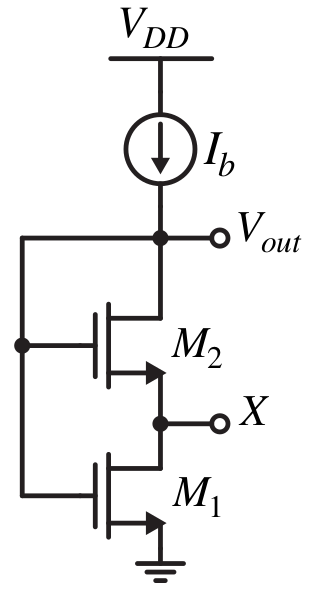
\includegraphics[width=.25\columnwidth]{p2a.png} \qquad\qquad & \qquad\qquad
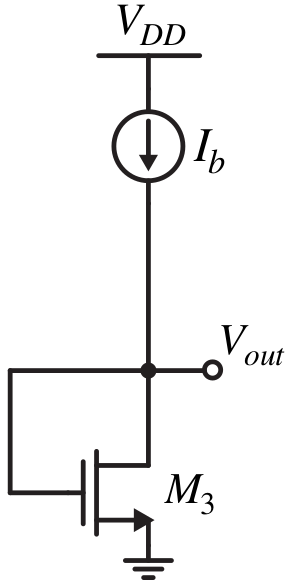
\includegraphics[width=.25\columnwidth]{p2b.png}\\
(a) \qquad\qquad & \qquad\qquad (b)\\
\end{tabular}
\caption{(a) Two $NMOS$ in series.  (b) A single diode-connected $NMOS$.}
\label{fig:circuits}
\end{figure}
%%%%%%%%%%%%%%%%%%%%%%%%%%%%%%%%%%%%%%%%%%%%
\noindent
\textbf{\emph{Find: }} The following:

\begin{enumerate}[label=(\alph*)]
    \item{For the circuit in \textit{Fig.~\ref{fig:circuits}a}, assume $I_D$ is large enough to bias $V_{out} > V_{Th}$, and ${\frac{W}{L}}_1 = {\frac{W}{L}}_2$. Determine the regions of operation for $M_1$ and $M_2$.}
    \item{For the circuit in \textit{Fig.~\ref{fig:circuits}b}, what value of ${\frac{W}{L}}_3$ will make it equivalent to the circuit in Fig.2.a? Express ${\frac{W}{L}}_3$ in terms of circuit parameters of $M_1$ and/or $M_2$.}
    \item{If we now consider the body effect, and given the sizing you found in part (b), which of the two circuits will have a higher output voltage, $V_{out}$? Assume that the body of all transistors is tied to ground. Explain your answer qualitatively (no math necessary).}
    \item{Find the value of the threshold voltage, $V_{th}$, for $M_1$ so that the node “X” in Fig.2.a has a potential of $V_{out} / 2$. Assume that $I_D$ is large enough to bias $V_{out} / 2 \cdot \max\{{V_{Th}}_1, {V_{Th}}_2\}$ and ${\frac{W}{L}}_1 = {\frac{W}{L}}_2$. Neglect the body effect as well as channel length modulation, and express your answer only in terms of $V_{out}$ and ${V_{Th}}_2\}$.}
\end{enumerate}

\newpage\noindent
\textbf{\emph{Solution: }}

\begin{enumerate}[label=(\alph*)]
    %%%%%%%%%%%%%%%%%%
    %%% SOLUTION A %%%
    %%%%%%%%%%%%%%%%%%
    \item
    {
        \textbf{Claim. } Transistor $M_2$ is in saturation, and transistor $M_1$ is in triode.
        \begin{proof}
            Since we are given $V_{out} > V_{Th}$, we can deduce that both transistors are on.  In the case of $M_1$ it is obvious because its source is connected to ground.  $M_2$ must also be on, because the constant current source $I_b$ biases it to ensure that there is a current.  Furthermore, $M_2$ is diode connected, so it must be in saturation.  Then we must somehow determine whether $M_1$ is in triode or saturation.
            
            We will proceed with a proof by contradiction.  Let's assume that both transistors are in saturation.  Then both of their drain currents must be equal.  Since the device parameters are equal, we have:
            \begin{align*}
                (V_{{GS}_1} - V_T) &= (V_{{GS}_2} - V_T)\\[0.25cm]
                (V_{out} - V_T) &= (V_{out} - V_X - V_T)\\[0.25cm]
                \implies 0 &= -V_X
            \end{align*}
            
            But we have already made it clear that $V_X$ cannot be $0\,V$, or else $M_2$ would be off, and $M_1$ would not be in saturation.  Thus, by contradiction we have proven that $M_2$ is in saturation, and $M_1$ is in triode.\\
        \end{proof}
    }
    \newpage
    %%%%%%%%%%%%%%%%%%
    %%% SOLUTION B %%%
    %%%%%%%%%%%%%%%%%%
    \item
    {
        First we can equate the saturation current of $M_2$ to the triode current of $M_1$:
        \begin{equation}
            \left({\frac{W}{2L}}_2\right)\,\mu\,C_{ox}{(V_{out} - V_X - {V_T})}^2 = \left({\frac{W}{L}}_1\right)\,\mu\,C_{ox}(V_{out} - V_T - \frac{{V_T}^2}{2})V_X
        \end{equation}
        The transistor parameters are equal, and we let $\phi = V_{out} - V_T$ to reduce the equation:
        \begin{align*}
            {(\phi - V_X)}^2 &= 2(\phi - \frac{V_X}{2})\\[0.25cm]
            \implies (\phi^2 - 2\phi V_X + {V_X}^2) &= 2\phi V_X - {V_X}^2\\[0.25cm]
            \implies 2 {V_X}^2 - 4\phi V_X + {\phi}^2 &= 0\\[0.25cm]
            \implies \underbrace{1}_A {V_X}^2) \underbrace{- 2\phi}_B V_X + \underbrace{\frac{1}{2}{\phi}^2}_C &= 0
        \end{align*}
        Solving the above quadratic equation yields two solutions:
        \begin{align}
            V_X &= \phi + \frac{\sqrt{{2\phi}^2}}{2}\\[0.25cm]
            V_X &= \phi - \frac{\sqrt{{2\phi}^2}}{2}
        \end{align}
        Now we can equate the saturation current of $M_2$ to the saturation current of $M_3$:
        \begin{equation}
            \left({\frac{W}{2L}}_2\right)\,\mu\,C_{ox}{(\phi - V_X)}^2) = \left({\frac{W}{2L}}_3\right)\,\mu\,C_{ox}\phi^2
        \end{equation}
        By inspection, we see that either solution will work, because the $\phi$'s will cancel out, leaving a single term inside of a square.  The using the first solution we have:
        \begin{align}
            \left({\frac{W}{2L}}_2\right)\,\bcancel{\mu\,C_{ox}}{\left(\cancel{\phi - \phi} + \frac{\sqrt{{2\phi}^2}}{2}\right)}^2 &= \left({\frac{W}{2L}}_3\right)\,\bcancel{\mu\,C_{ox}}\phi^2\\[0.25cm]
            \implies \left({\frac{W}{L}}_2\right)\,\left(\frac{1}{2}\phi^2 \right) &= \left({\frac{W}{2L}}_3\right)\,\phi^2
        \end{align}
        Finally, we see that:
        \begin{equation}
            \boxed{\left({\frac{W}{L}}_2\right)\,\left(\frac{1}{2}\right) = \left({\frac{W}{2L}}_3\right)}
        \end{equation}
    }
    %%%%%%%%%%%%%%%%%%
    %%% SOLUTION C %%%
    %%%%%%%%%%%%%%%%%%
    \item{With a body effect, transistors $M_3$ and $M_1$ will be unaffected, because their source is tied to ground.  However, transistor $M_2$'s source is at node $V_X$, and thus $V_{SB} > 0$.  This means that the effective threshold voltage will increase.  But the current source still biases the drain current, so it must remain the same.  Thus, the gate voltage must increase to compensate for this change.}
    \newpage
    %%%%%%%%%%%%%%%%%%
    %%% SOLUTION D %%%
    %%%%%%%%%%%%%%%%%%
    \item
    {
    We can equate the triode current of $M_1$ to the saturation current of $M_2$, knowing that their device parameters are equivalent except for a factor of 2.  We will again let $\phi_1 = V_{out} - V_{{Th}_1}$ and $\phi_2 = V_{out} - V_{{Th}_2}$.  Then we have:
    \begin{align*}
        \cancel{\left({\frac{W}{L}}_1\,\mu C_{ox}\right)}\left(\phi_1 - \frac{{V_X}^2}{2}\right)\,V_X &= \frac{1}{2}\cancel{\left({\frac{W}{L}}_2\,\mu C_{ox}\right)}{(\phi_2 - V_X)}^2\\[0.25cm]
        2\left(\phi_1 V_X - \frac{{V_X}^2}{2}\right) &= \phi_2 - 2\phi_2 V_X + {V_X}^2\\[0.25cm]
        2\left[\phi_1 \frac{V_{out}}{2} - \frac{1}{2} {\left(\frac{V_{out}}{2}\right)}^2\right] &= \phi_2 - 2\phi_2\left(\frac{V_{out}}{2}\right) + {\left(\frac{V_{out}}{2}\right)}^2\\[0.25cm]
        \phi_1 V_{out} - \frac{{V_{out}}^2}{4} &= \phi_2 - \phi_2 V_{out} + \frac{{V_{out}}^2}{4}\\[0.25cm]
        \phi_1 V_{out} &= \phi_2(1 - V_{out}) + \frac{{V_{out}}^2}{2}\\[0.25cm]
        \phi_1 &= \phi_2\left(\frac{1}{V_{out}} - 1\right) + \frac{V_{out}}{2}
    \end{align*}
    Plugging back in our substitutions for $\phi_1$ and $\phi_2$, and simplifying yields the answer:
    \begin{align*}
        V_{out} - V_{{Th}_1} &= V_{out} - V_{{Th}_2}\left(\frac{1}{V_{out}} - 1\right) + \frac{V_{out}}{2}\\[0.25cm]
        -V_{{Th}_1} &= V_{{Th}_2}\left(1 - \frac{1}{V_{out}}\right) + \frac{V_{out}}{2}\\[0.25cm]
        \implies \Aboxed{V_{{Th}_1} &= -V_{{Th}_2}\left(1 - \frac{1}{V_{out}}\right) - \frac{V_{out}}{2}}
    \end{align*}
    }
\end{enumerate}
%%%%%%%%%%%%%%%%%%%%%%%%%%%%%%%%%%%%%%%%%%%%%%%%%%%%%%%%%%%%%%%%%%%%%%%%%%%%%%%%%%%%%%%%%%%%%%%%%%%%%%%%%%%
%                                           QUESTION 3                                                    %
%%%%%%%%%%%%%%%%%%%%%%%%%%%%%%%%%%%%%%%%%%%%%%%%%%%%%%%%%%%%%%%%%%%%%%%%%%%%%%%%%%%%%%%%%%%%%%%%%%%%%%%%%%%
\newpage
\section{Velocity Saturation}
\textbf{\emph{Given: }} The following circuit, with the following set of parameters.  You may neglect channel length modulation for all large signal calculations.\\[0.25cm]
    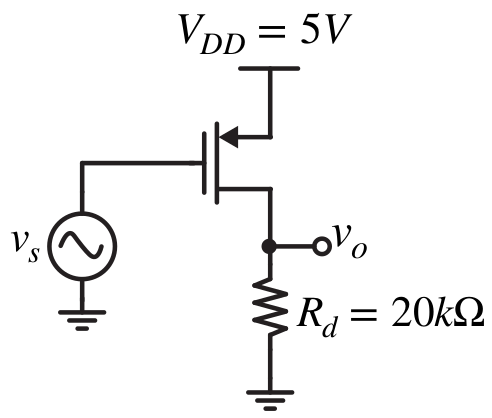
\includegraphics[scale=0.45, center]{p3.png}\\
    \begin{table}[H]
    \centering
    \setlength{\tabcolsep}{20pt}
    \renewcommand{\arraystretch}{1.5}
        \begin{tabular}{|l|c|}
            \hline
            $W$ & $5\,\mu m$\\
            \hline
            $L$ & $1\,\mu m$\\
            \hline
            $\mu C_{ox}$ & $150\,\mu A/V^2$\\
            \hline
            $\lambda$ & $0.02\,V^{-1}$\\
            \hline
            $\left|V_{th}\right|$ & $0.8\,V$\\
            \hline
        \end{tabular}
    \end{table}

\noindent
\textbf{\emph{Find: }} The following:

\begin{enumerate}[label=(\alph*)]
    \item{If the input is biased at $3.5\,V$, calculate $g_m$ and $r_o$ for the device.}
    \item{Draw the small signal model for the circuit.}
    \item{Using nodal analysis, compute the small-signal gain, $A_v = v_o / v_s$.}
    \item{Now the replace the device with a short channel one with $W/L = 250\,nm / 50\,nm$. We would like to consider the effect of velocity saturation.  Derive a symbolic expression for the transconductance of a velocity saturated $PMOS$, assuming that ${V_{DS}}_{sat} = L \cdot \mathcal{E}_{sat}$.}
    \item{Using the formula you derived, calculate the value of $g_m$ for the $PMOS$ device mentioned in part (d). Assume that $\mathcal{E}_{sat} = 50\,kV \cdot cm^{-1}$.}
    \item{With $r_o \gg R_d$, redo part (c) for the modified circuit. This is not a good assumption, but we will leave calculating $r_o$ to a circuit simulator.}
\end{enumerate}

\newpage\noindent
\textbf{\emph{Solution: }}

\noindent
The transistor is a $PMOS$ amplifier in a common-drain (source follower) configuration.  Before solving for any small-signal parameters we must first figure out the operating region of the transistor.

Since $V_{SG} = 1.5\,V > V_T = 0.8\,V$, we know that it is on.  We will assume saturation and see if that assumption is valid.  The drain current across the resistor is equal to the saturation current, and it is:
    \begin{equation}
        I_D = \frac{V_D}{R_d}
        \label{eq:id_rd_vd}
    \end{equation}
We are given everything to solve for the saturation current:
    \begin{align*}
        I_{D} &= \left(\frac{W}{2L}\right) \mu_p\,C_{ox} {\big(V_{SG} - \left|V_{T_p}\right|\big)}^2\\[0.25cm]
        &= \left(\frac{5}{2}\right) 150\,\mu A/V^2 {\big(1.5\,V - 0.8\,V\big)}^2\\[0.25cm]
        &= 183.75\,\mu A = 0.18375\,mA
    \end{align*}
Rearranging \textit{Eq.~\ref{eq:id_rd_vd}} to solve for the drain voltage:
    \begin{equation}
        V_D = I_D\,R_d = (0.18375\,mA)(20k\,\Omega) = 3.675\,V
    \end{equation}
Now that we have found the drain voltage, we see that $V_{SD} = 5\,V - 3.675\,V = \boxed{1.325\,V} > V_{OV}$, and indeed the transistor is in saturation.  We will now proceed with all sub-problems since we know the region of operation.
\newpage
\begin{enumerate}[label=(\alph*)]
    %%%%%%%%%%%%%%%%%%
    %%% SOLUTION A %%%
    %%%%%%%%%%%%%%%%%%
    \item
    {
    Now that we have confirmed that the device is in saturation, we can use the first form of \textit{Eq.~\ref{eq:mos_transconductance}} to solve for the small-signal parameters.  Starting with the transconductance:
    \begin{align*}
        g_m &= \left(\frac{W}{L}\right)\mu\,C_{ox}(V_{SG} - \left|V_{T_p}\right|))\\[0.25cm]
        &= \frac{5\,\cancel{\mu m}}{1\,\cancel{\mu m}} \cdot 150\,\mu A/V^2 \cdot (1.5\,V - 0.8\,V)\\[0.25cm]
        &= 750\,\mu A/V^2 \cdot (0.7\,V)\\[0.25cm]
        &= 525\,\left(\frac{\mu A}{V^{\cancel{2}}}\right)(\cancel{V})\\[0.25cm]
        &= 525\,\frac{\mu A}{V} = 525\,\mu S\\[0.25cm]
        \Aboxed{g_m &= 0.525\,mS}
    \end{align*}
    }
    
    Now with reference to \textit{Eq.~\ref{eq:mos_outresistance}} we solve for the output resistance:
    \begin{align*}
        r_o &= \mathlarger{\frac{1}{\frac{W\,\mu\,C_{ox}}{2L}{(V_{SG} - \left|V_T\right|)}^2\,\lambda}}\\[0.25cm]
        &= \frac{1}{375\,\mu A/V^2{(0.7\,V)}^2\,(0.02\,V^{-1})}\\[0.25cm]
        &= \frac{V}{3.675\,\mu A} = \frac{V}{\num{3.675e-6}\,A}\\[0.25cm]
        &= 272108.8435\,\Omega\\[0.25cm]
        \Aboxed{r_o &\approx 272\,k \Omega}
    \end{align*}
    \newpage
    %%%%%%%%%%%%%%%%%%
    %%% SOLUTION B %%%
    %%%%%%%%%%%%%%%%%%
    \item
    {
    Below is the small-signal model of the circuit, with all $DC$ sources turned off.
    %%%%%%%%%%%%%%%%%%%%%%%%%%%%%%%%%%%%%%%%%%%%
    %                 FIGURE                   %
    %%%%%%%%%%%%%%%%%%%%%%%%%%%%%%%%%%%%%%%%%%%%
    \begin{figure}[H]
    \centering
    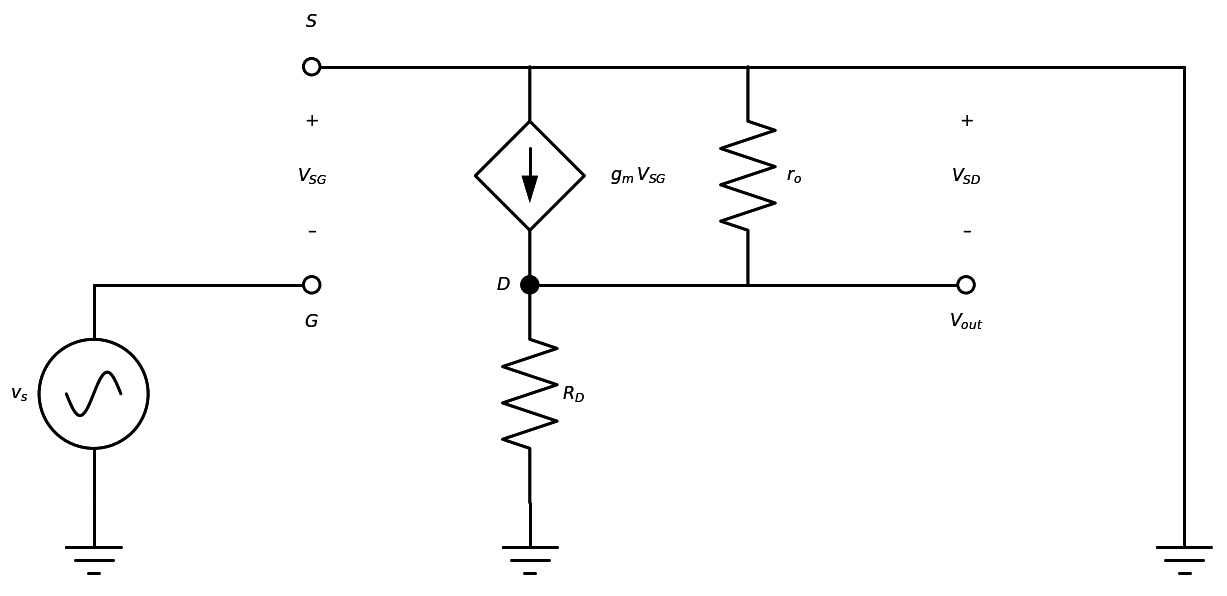
\includegraphics[scale=0.4]{p3b.png}
    \caption{The small-signal circuit model.}
    \label{fig:small_signal}
    \end{figure}
    %%%%%%%%%%%%%%%%%%%%%%%%%%%%%%%%%%%%%%%%%%%%
    }
    %%%%%%%%%%%%%%%%%%
    %%% SOLUTION C %%%
    %%%%%%%%%%%%%%%%%%
    \item
    {
    KCL at the drain node yields:
    \begin{align*}
        \frac{V_D}{R_D} + \frac{V_D - \cancelto{0}{V_S}}{r_o} &= g_m\,V_{SG}
        = \cancelto{0}{g_m\,V_S} - g_m\,V_G\\[0.25cm]
        &\Longrightarrow V_D\left(\frac{1}{R_D} + \frac{1}{r_o}\right) = -g_m\,V_G
    \end{align*}
    The gate voltage is equal to the sinusoidal source input, and the drain voltage is the output.  Rearranging the above equation gives us a symbolic expression for the small-signal gain:
    \begin{equation*}
        \boxed{\frac{V_D}{V_G} = \frac{v_{out}}{v_s} = -g_m\,(R_D \parallel r_o)}
    \end{equation*}
    Plugging in numbers to obtain a value yields:
    \begin{align*}
        A_v &=  -(0.525\,mS)\,\left(\frac{20000\,\Omega \cdot 272108.8435\,\Omega}{20000\,\Omega + 272108.8435\,\Omega}\right)\\[0.25cm]
        \Aboxed{&=-9.781089893 \approx -9.8}
    \end{align*}
    }
    \newpage
    %%%%%%%%%%%%%%%%%%
    %%% SOLUTION D %%%
    %%%%%%%%%%%%%%%%%%
    \item
    {
    We can take the derivative of the saturation current equation with respect to $V_{SG}$ to get the transconductance of a short-channel device.  We will take the channel-length modulation into consideration since this is a small-signal parameter:
    
    \begin{align*}
        g_m &= \frac{d}{dV_{SG}}\left[\left(\frac{W}{2L}\right) \mu_p\,C_{ox} {\big(V_{SG} - \left|V_{T_p}\right|\big)}^2 (1 + \lambda V_{SD})\right]\\[0.25cm]
        &= \frac{d}{dV_{SG}}\left[\left(\frac{W}{2L}\right) \mu_p\,C_{ox} \big(V_{SG} - \left|V_{T_p}\right|\big)\,V_{{SD}_{sat}} (1 + \lambda V_{SD})\right]\\[0.25cm]
        &= \frac{W}{2L}\,\mu\,C_{ox}2(V_{SG} - \left|V_T\right|)(1 + \lambda V_{SD})\\[0.25cm]
        &= \frac{W}{2L}\,\mu\,C_{ox}(V_{{SD}_{sat}})(1 + \lambda V_{SD})\\[0.25cm]
    \end{align*}
    When we substitute the field for the saturation drain voltage, the length cancels and we have found the symbolic expression:
    \begin{equation}
        \boxed{g_m = \frac{W}{2}\,\mu\,C_{ox}\mathcal{E}(1 + \lambda V_{SD})}
    \end{equation}
    }
    %%%%%%%%%%%%%%%%%%
    %%% SOLUTION E %%%
    %%%%%%%%%%%%%%%%%%
    \item
    {
    Plugging in all the known values for the numerical answer:
    \begin{align*}
        g_m &= (125\,nm)\left(\frac{1\,m}{10^9\,nm}\right)\left(\frac{100\,cm}{1\,m}\right)(150\,\mu A/V^2)\left(\frac{50\,kV}{cm}\right)\Big(1 + (0.02V^{-1}(1.325\,V)\Big)\\[0.25cm]
        &= 96.234375\,\mu S\\[0.25cm]
        \Aboxed{&\approx 0.96\,mS}
    \end{align*}
    }
    %%%%%%%%%%%%%%%%%%
    %%% SOLUTION F %%%
    %%%%%%%%%%%%%%%%%%
    \item
    {
    With $r_o \gg R_D$, the drain resistor dominates, and our gain is simply $-g_m\,R_D$.  Plugging in for a numerical value:
    \begin{equation}
        A_v = -g_m\,R_D = -(\num{0.192e-3}\,mS)(20k\,\Omega) = -1.9246875 \boxed{\approx -1.9}
    \end{equation}
    }
\end{enumerate}
%%%%%%%%%%%%%%%%%%%%%%%%%%%%%%%%%%%%%%%%%%%%%%%%%%%%%%%%%%%%%%%%%%%%%%%%%%%%%%%%%%%%%%%%%%%%%%%%%%%%%%%%%%%
%                                             APPENDIX                                                    %
%%%%%%%%%%%%%%%%%%%%%%%%%%%%%%%%%%%%%%%%%%%%%%%%%%%%%%%%%%%%%%%%%%%%%%%%%%%%%%%%%%%%%%%%%%%%%%%%%%%%%%%%%%%
\appendix
%%%%%%%%%%%%%%%%%%%%%%%%%%%%%%%%%%%%%%%%%%%%%%%%%%%%%%%%%%%%%%%%%%%%%%%%%%%%%%%%%%%%%%%%%%%%%%%%%%%%%%%%%%%
%                                APPENDIX A: GLOSSARY OF EQUATIONS                                        %
%%%%%%%%%%%%%%%%%%%%%%%%%%%%%%%%%%%%%%%%%%%%%%%%%%%%%%%%%%%%%%%%%%%%%%%%%%%%%%%%%%%%%%%%%%%%%%%%%%%%%%%%%%%
\newpage
\section{Appendix: Glossary of Equations}
    \begin{flalign}
        &&\Aboxed{\phi_{bi} &= \frac{kT}{q} \cdot ln\;\bigg( \frac{N_D \cdot N_A}{{n_i}^2} \bigg)}
        &&\textit{Built-in potential, $PN$-junction}
        \label{eq:phi_bi}
    \end{flalign}

    \begin{flalign}
        &&\Aboxed{W_{dep} &= \sqrt{\frac{2\epsilon_s \left(\phi_{bi} - V_{applied}\right)}{q}
                        \cdot \Bigg( \frac{1}{N_A} + \frac{1}{N_D} \Bigg)}}
        &&\textit{Depletion region width, total}
        \label{eq:total_dep}
    \end{flalign}        

    \begin{flalign}
        &&\Aboxed{C_{dep} &= A \left(\frac{\epsilon_s}{W_{dep}}\right)}
        &&\textit{Junction capacitance}
        \label{eq:junc_cap}
    \end{flalign}

    \begin{flalign}
        &&\Aboxed{I_{DS,sat} &= \left(\frac{W}{2L}\right) \mu_n\,C_{ox}
                         {\big(V_{GS} - V_{T_n}\big)}^2 (1 + \lambda V_{DS})}
        &&\textit{$NMOS$ saturation current}
        \label{eq:mosfet_ids_nmos_sat}\\[0.25cm]
        &&\Aboxed{I_{DS,tri} &= \left(\frac{W}{L}\right) \mu_n\,C_{ox}
                            \left(V_{GS} - V_{T_n} - \frac{V_{DS}}{2}\right) V_{DS}}
        &&\textit{$NMOS$ triode current}
        \label{eq:mosfet_ids_nmos_tri}\\[0.25cm]
        &&\Aboxed{I_{SD,sat} &= \left(\frac{W}{2L}\right) \mu_p\,C_{ox}
                         {\big(V_{SG} - \left|V_{T_p}\right|\big)}^2 (1 + \lambda V_{SD})}
        &&\textit{$PMOS$ saturation current}
        \label{eq:mosfet_ids_pmos_sat}\\[0.25cm]
        &&\Aboxed{I_{SD,tri} &= \left(\frac{W}{L}\right) \mu_p\,C_{ox}
                            \left(V_{SG} - \left|V_{T_p}\right| - \frac{V_{SD}}{2}\right) V_{SD}}
        &&\textit{$PMOS$ triode current}
        \label{eq:mosfet_ids_pmos_tri}
    \end{flalign}

    \begin{flalign}
        &&\Aboxed{r_o &= \frac{1}{\frac{W\,\mu\,C_{ox}}{2L}{(V_{GS} - V_T)}^2\,\lambda}
        \approx \frac{1}{\lambda\,I_{DS}}}
        &&\textit{Output resistance for MOSFET}
        \label{eq:mos_outresistance}
    \end{flalign}

    \begin{flalign}
        &&\Aboxed{g_m &= \left(\frac{W}{L}\right)\mu\,C_{ox}(V_{{DS}_{sat}})
        = \sqrt{\left(\frac{2W}{L}\right)\mu\,C_{ox} I_{DS}}
        = \frac{2 \cdot I_{DS}}{V_{GS} - V_T}}
        &&\textit{Transconductance for MOSFET}
        \label{eq:mos_transconductance}
    \end{flalign}

    \begin{flalign}
        &&\Aboxed{V_{GS} = V_T + \sqrt{\frac{2\,I_{DS}}{\frac{W}{L} \mu C_{ox}}} = V_T + V_{OD}}
        &&\textit{Gate-source condition, diode-connected MOSFET}
        \label{eq:mos_gate_cond}
    \end{flalign}
%%%%%%%%%%%%%%%%%%%%%%%%%%%%%%%%%%%%%%%%%%%%%%%%%%%%%%%%%%%%%%%%%%%%%%%%%%%%%%%%%%%%%%%%%%%%%%%%%%%%%%%%%%%
%                                APPENDIX B: GLOSSARY OF TABLES                                           %
%%%%%%%%%%%%%%%%%%%%%%%%%%%%%%%%%%%%%%%%%%%%%%%%%%%%%%%%%%%%%%%%%%%%%%%%%%%%%%%%%%%%%%%%%%%%%%%%%%%%%%%%%%%
\newpage
\section{Appendix: Glossary of Tables}
    \begin{table}[H]
    \centering
    \setlength{\tabcolsep}{20pt}
    \renewcommand{\arraystretch}{1.5}
    \begin{tabular}{|l|c|c|c|}
        \hline
        \textbf{Transistor Type}  &  \textbf{Cut-off} & \textbf{Triode} & \textbf{Saturation}\\
        \hline
        \textit{NMOS} & $V_{GS} \leq V_{T_n}$
                        & $V_{DS} \leq V_{GS} - V_{T_n}$
                        & $V_{DS} > V_{GS} - V_{T_n}$\\
        \hline
        \textit{PMOS} & $V_{SG} \leq \left|V_{T_p}\right|$
                        & $V_{SD} \leq V_{SG} - \left|V_{T_p}\right|$
                        & $V_{SD} > V_{SG} - \left|V_{T_p}\right|$\\
        \hline
    \end{tabular}
    \caption{Conditions for MOSFET regions of operation.
    \label{tab:mosfet_op}} 
    \end{table}

    \begin{table}[H]
    \centering
    \setlength{\tabcolsep}{20pt}
    \renewcommand{\arraystretch}{1.5}
    \begin{tabular}{|l|c|c|}
        \hline
        \textbf{Description}  &  \textbf{Symbol} & \textbf{Value}\\
        \hline
        Elementary charge & $q$ & $\num{1.60218e-19}\,C$\\
        \hline
        Electron volt & $eV$ & $\num{1.60218e-19}\,J$\\
        \hline
        Boltzmann's constant & $k$ & $\num{1.38066e-23}\,J/K$\\
        \hline
        Free electron mass & $m_0$ & $\num{9.1095e-31}\,kg$\\
        \hline
        Permittivity in vacuum & $\epsilon_0$ & $\num{8.85418e-12}\,F/m$\\
        \hline
        Planck's constant & $h$ & $\num{6.62617e-34}\,J \cdot s$\\
        \hline
        Reduced Planck's constant ($h/2\pi$) & $\hbar$ & $\num{1.05458e-34}\,J \cdot s$\\
        \hline
        Speed of light in vacuum & $c$ & $\num{2.99792e8}\,m/s$\\
        \hline
        Thermal voltage at $T=300^{\circ}K$ & $kT/q$ & $0.0259\,V$\\
        \hline
        Wavelength of 1-$eV$ photon & $\lambda$ & $1.23977\,\mu m$\\
        \hline
    \end{tabular}
    \caption{Physical constants.
    \label{tab:phys_const}} 
    \end{table}
\newpage
    \begin{table}[H]
    \centering
    \setlength{\tabcolsep}{20pt}
    \renewcommand{\arraystretch}{1.5}
    \begin{tabular}{|l|c|c|}
        \hline
        \textbf{Quantity}  &  \textbf{Symbol} & \textbf{Value/Dimension}\\
        \hline
        Meter & $m$ & $1\,m = 10^2\,cm$\\
        \hline
        Millimeter & $mm$ & $1\,mm = 10^{-1}\,cm = 10^{-3}\,m$\\
        \hline
        Micrometer, micron & $\mu m$ & $1\,\mu m = 10^4\,\text{\AA} = 10^3\,mm = 10^{-4}\,cm$\\
        \hline
        Nanometer & $nm$ & $1\,nm = 10\,\text{\AA} = 10^{-3}\,\mu m = 10^{-7}\,cm$\\
        \hline
        Angstrom & $\text{\AA}$ & $1\,\text{\AA} = 10^{-4}\,\mu m = 10^{-8}\,cm = 10^{-10}\,m$\\
        \hline
        Electron volt & $eV$ & $1\,eV = \num{1.60218e-19}\,J$\\
        \hline
        Electric charge (Coulomb) & $C$ & $A \cdot s$\\
        \hline
        Current (Ampere) & $A$ & $C/s$\\
        \hline
        Frequency (Hertz) & $Hz$ & $1/s$\\
        \hline
        Energy (Joule) & $J$ & $N \cdot m$\\
        \hline
        Power (Watt) & $W$ & $J/s$\\
        \hline
        Potential (Volt) & $V$ & $J/C$\\
        \hline
        Conductance (Siemens) & $S$ & $A/V$\\
        \hline
        Resistance (Ohm) & $\Omega$ & $V/A$\\
        \hline
        Capacitance (Farad) & $F$ & $C/V$\\
        \hline
    \end{tabular}
    \caption{Unit conversions.
    \label{tab:unit_conv}} 
    \end{table}
\newpage
%%%%%%%%%%%%%%%%%%%%%%%%%%%%%%%%%%%%%%%%%%%%%%%%%%%%%%%%%%%%%%%%%%%%%%%%%%%%%%%%%%%%%%%%%%%%%%%%%%%%%%%%%%%
%                                           BIBLIOGRAPHY                                                  %
%%%%%%%%%%%%%%%%%%%%%%%%%%%%%%%%%%%%%%%%%%%%%%%%%%%%%%%%%%%%%%%%%%%%%%%%%%%%%%%%%%%%%%%%%%%%%%%%%%%%%%%%%%%
\newpage
\addcontentsline{toc}{section}{References}
\emergencystretch=2em
\nocite{*}
\printbibliography
%%%%%%%%%%%%%%%%%%%%%%%%%%%%%%%%%%%%%%%%%%%%%%%%%%%%%%%%%%%%%%%%%%%%%%%%%%%%%%%%%%%%%%%%%%%%%%%%%%%%%%%%%%%
%                                           END OF DOCUMENT                                               %
%%%%%%%%%%%%%%%%%%%%%%%%%%%%%%%%%%%%%%%%%%%%%%%%%%%%%%%%%%%%%%%%%%%%%%%%%%%%%%%%%%%%%%%%%%%%%%%%%%%%%%%%%%%
\end{document}
